\documentclass{article}
\usepackage{cmap}
\usepackage[utf8]{inputenc}
\usepackage[english,ukrainian]{babel}
\usepackage{graphicx}
\usepackage{geometry}
\usepackage{listings}
\usepackage{float}
\geometry{
	a4paper,
	left=20mm,
	right=20mm,
	top=20mm,
	bottom=20mm
}
\lstset{
	language=c,
	tabsize=4,
	keepspaces,
	showstringspaces=false,
}
\graphicspath{ {./pictures} }
\setlength{\parindent}{4em}

\newcommand\subject{Алгоритми та структури даних}
\newcommand\lecturer{доцент кафедри ПЗ\\Коротєєва Т.О.}
\newcommand\teacher{асистент кафедри ПЗ\\Франко А.В.}
\newcommand\mygroup{ПЗ-22}
\newcommand\lab{2}
\newcommand\theme{Метод сортування вибором}
\newcommand\purpose{Вивчити алгоритм сортування вибором. Здійснити програмну реалізацію алгоритму сортування вибором. Дослідити швидкодію алгоритму сортування вибором}

\begin{document}
	\begin{normalsize}
		\begin{titlepage}
			\thispagestyle{empty}
			\begin{center}
				\textbf{МІНІСТЕРСТВО ОСВІТИ І НАУКИ УКРАЇНИ\\
					НАЦІОНАЛЬНИЙ УНІВЕРСИТЕТ "ЛЬВІВСЬКА ПОЛІТЕХНІКА"}
			\end{center}
			\begin{flushright}
				Інститут \textbf{КНІТ}\\
				Кафедра \textbf{ПЗ}
			\end{flushright}
			\vspace{200pt}
			\begin{center}
				\textbf{ЗВІТ}\\
				\vspace{10pt}
				До лабораторної роботи № \lab\\
				\textbf{На тему}: “\textit{\theme}”\\
				\textbf{З дисципліни}: “\subject”
			\end{center}
			\vspace{112pt}
			\begin{flushright}
				
				\textbf{Лектор}:\\
				\lecturer\\
				\vspace{28pt}
				\textbf{Виконав}:\\
				
				студент групи \mygroup\\
				Коваленко Д.М.\\
				\vspace{28pt}
				\textbf{Прийняв}:\\
				
				\teacher\\
				
				\vspace{28pt}
				«\rule{1cm}{0.15mm}» \rule{1.5cm}{0.15mm} 2022 р.\\
				$\sum$ = \rule{1cm}{0.15mm}……………\\
				
			\end{flushright}
			\vspace{\fill}
			\begin{center}
				\textbf{Львів — 2022}
			\end{center}
		\end{titlepage}
		
		\begin{description}
			\item[Тема.] \theme.
			\item[Мета.] \purpose.
		\end{description}
		
		\section*{Лабораторне завдання}
		Створити віконний проект та написати програму, яка реалізує алгоритм сортування бульбашкою.
		\begin{center}
			3. Задано одномірний масив дійсних чисел. До парних елементів масиву застосувати функцію $\sqrt{|x-10|}$. Отриманий масив посортувати в порядку зростання
		\end{center}
		
		\section*{Теоретичні відомості}
		Сортування вибором (англійською «Selection Sort») — простий алгоритм сортування лінійного масиву, на основі вставок. Має ефективність O(n2), що робить його неефективним при сортування великих масивів, і в цілому, менш ефективним за подібний алгоритм сортування включенням. Сортування вибором вирізняється більшою простотою, ніж cортування включенням, і в деяких випадках вищою продуктивністю.
		
		Алгоритм працює наступним чином:
		
		1.     Знаходить у списку найменше значення.
		
		2.     Міняє його місцями із першим значеннями у списку.
		
		3.     Повторює два попередніх кроки, доки список не завершиться (починаючи з другої позиції).
		
		Фактично, таким чином ми поділили список на дві частини: перша (ліва) — повністю відсортована, а друга (права) — ні.
		
		\subsection*{Покроковий опис роботи алгоритму сортування вибором}
		\textbf{Алгоритм S}
		
		S1 - встановити MIN = 0
		
		S2 - знайти найменший елемент в масиві
		
		S3 - замінити найменший елемент на той, що розміщений на місці MIN
		
		S4 - збільшити значення MIN на 1
		
		S5 - повторити виконання S2 - S4
		
		
		\section*{Хід роботи}
		\subsection*{Файл sort.rs}
		\begin{lstlisting}
use crate::data::Data;

pub struct Sorted;

impl Sorted {
	pub fn sort(mut v: Vec<Data>) -> Vec<Vec<Data>> {
		let mut res = vec![v.clone()];
		for i in 0..(v.len() - 1) {
			let mut min = i;
			for j in (i + 1)..v.len() {
				if v[j] < v[min] {
					min = j;
				}
			}
			if min != i {
				v.swap(i, min);
				res.push(v.clone());
			}
		}
		res
	}
}
\end{lstlisting}
		\subsection*{Файл data.rs}
		\begin{lstlisting}
use fake::{Dummy, Fake};

#[derive(Debug, Clone, PartialEq, Dummy)]
pub struct Data {
	#[dummy()]
	pub v: f32,
}

impl Data {
	pub fn new(len: usize) -> Vec<Self> {
		let mut vec = fake::vec![Data; len];
		vec.iter_mut()
		.step_by(2)
		.for_each(|x| x.v = f32::sqrt(f32::abs(x.v - 10.)));
		vec
	}
	
	pub fn diff(a: &Vec<Data>, b: &Vec<Data>) -> Vec<usize> {
		let mut res = Vec::new();
		
		for i in 0..a.len() {
			if a[i] != b[i] {
				res.push(i);
			}
		}
		
		res
	}
}

impl PartialOrd for Data {
	fn partial_cmp(&self, other: &Self) -> Option<std::cmp::Ordering> {
		self.v.partial_cmp(&other.v)
	}
}\end{lstlisting}
		\subsection*{Файл lib.rs}
		\begin{lstlisting}
extern crate console_error_panic_hook;

mod data;
mod sort;
mod utils;

use wasm_bindgen::{prelude::*, JsCast};
use web_sys::{
	HtmlElement, HtmlInputElement, 
	HtmlTableCellElement, HtmlTableElement, 
	HtmlTableRowElement,
	Text,
};

use data::Data;
use utils::document;
use sort::Sorted;

use std::{cell::RefCell, rc::Rc};

use std::panic;

#[wasm_bindgen]
extern "C" {
	#[wasm_bindgen(js_namespace = console)]
	fn log(s: &str);
}

#[wasm_bindgen(start)]
pub fn run() {
	panic::set_hook(Box::new(console_error_panic_hook::hook));
	
	let slider = Rc::new(RefCell::new(
	document()
	.get_element_by_id("slider")
	.unwrap()
	.dyn_into::<HtmlInputElement>()
	.unwrap(),
	));
	let slider_onchange = slider.clone();
	let f = Closure::wrap(Box::new(move || {
		let len = slider_onchange.borrow().value_as_number();
		document()
		.get_element_by_id("slider_value")
		.unwrap()
		.dyn_into::<HtmlElement>()
		.unwrap()
		.set_inner_html(&len.to_string());
		let data = Sorted::sort(Data::new(len as usize));
		let table = document()
		.get_element_by_id("table")
		.unwrap()
		.dyn_into::<HtmlTableElement>()
		.unwrap();
		table.set_inner_html("");
		for i in 0..data.len() {
			let diff = if let Some(b) = data.get(i + 1) {
				Data::diff(&data[i], &b)
			} else {
				vec![100, 100]
			};
			let row = table
			.insert_row()
			.unwrap()
			.dyn_into::<HtmlTableRowElement>()
			.unwrap();
			for j in 0..data[i].len() {
				let cell = row
				.insert_cell()
				.unwrap()
				.dyn_into::<HtmlTableCellElement>()
				.unwrap();
				let text = document()
				.create_text_node(&data[i][j].v.to_string())
				.dyn_into::<Text>()
				.unwrap();
				cell.append_child(&text).unwrap();
				if diff.contains(&j) {
					cell.set_bg_color("rgb(255,200,200)");
				}
			}
		}
	}) as Box<dyn FnMut()>);
	slider
	.borrow()
	.set_oninput(Some(f.as_ref().unchecked_ref()));
	f.forget();
}\end{lstlisting}
		
		\begin{figure}[H]
			\centering
			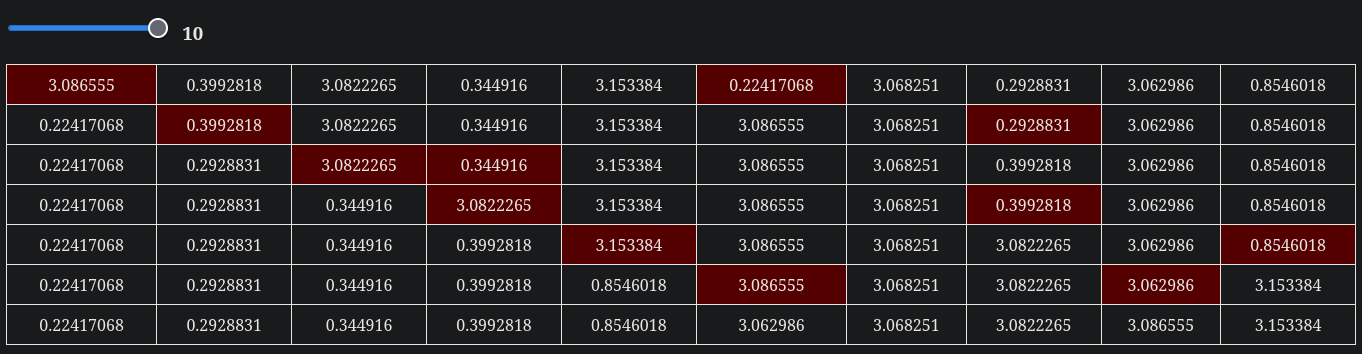
\includegraphics[scale=0.36]{1}
			\caption{Виконання програми}
		\end{figure}
		
		\section*{Висновок}
		Під час виконяння лабораторної роботи я вивчив алгоритм сортування вибором. Здійснив програмну реалізацію алгоритму сортування вибором. Дослідив швидкодію алгоритму сортування вибором.
		
	\end{normalsize}
\end{document}
